% !TeX root = ../../main.tex
\graphicspath{{Parts/3_Integrations/graphics/}}
\subsection{Overleaf}
The best way to use local \LaTeX{} is \emph{in conjunction with}, and not instead of Overleaf. Overleaf does have its own strengths after all, due to its real time collaboration ability. Overleaf and local versions of \LaTeX{} can be integrated into one seamless experience using Github (although, the owner of the document must have Overleaf premium for this feature). This can be done as follows
\begin{enumerate}
    \item Have your \LaTeX{} project in a Github repository. It is fine if your repo consists of other files such as project code, but keep in mind that Overleaf project sizes are limited to 100MB. If the Github repo for your project is larger than this, then it is probably better to save your writeup as a submodule in the project repository (and use this submodule as the repository for the \LaTeX{} project itself).
    \item Now, when creating a new project, select the option to import from Github
    \begin{figure}[ht!]
        \centering
        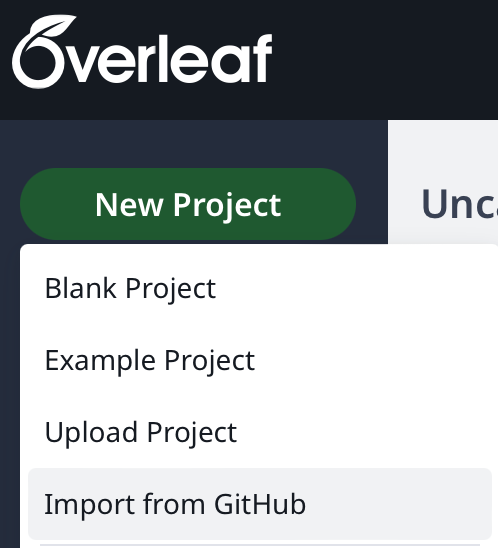
\includegraphics[width = 0.4\textwidth]{new}
        \caption{Importing a project from Github}
    \end{figure}
\end{enumerate}